\begin{figure}[H]
    \center
    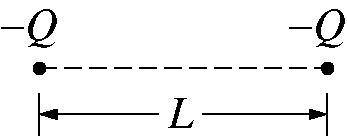
\includegraphics[scale=0.25]{images/img-007-015.png}
\end{figure}

% Multiple Choice Question 18
\begin{questions}\setcounter{question}{17}\question
Two particles each with a charge $-Q$ are fixed a distance $L$ apart as shown above. Each particle experiences a net electric force $F$. A particle with a charge $+q$ is now fixed midway between the original two particles. As a result, the net electric force experienced by each negatively charged particle is reduced to $F / 2$. The value of $q$ is

\begin{oneparchoices}
\choice $Q$
\choice $\dfrac{Q}{2} $
\choice $\dfrac{Q}{4} $
\choice $\dfrac{Q}{8} $
\choice $\dfrac{Q}{16}$
\end{oneparchoices}\end{questions}

